\documentclass[biblatex, charis, linguex]{glossa}

\bibliography{rs} 

\usepackage{sectsty} 
\allsectionsfont{\normalfont\sffamily\bfseries}
\subsectionfont{\normalfont\sffamily\bfseries\itshape}
\let\B\relax 
\let\T\relax
\usepackage[linguistics]{forest}

\pdfauthor{Roland Schaefer and Elizabeth Pankratz}
\pdftitle{On the transparency of N-N compounds: Pluralic linking elements in German can have plural semantics}
\pdfkeywords{usage-based grammar, word formation, linking elements, split-100 experiments, corpus data, German}

\title[On the transparency of N-N compounds]{On the transparency of N-N compounds: Pluralic linking elements in German can have plural semantics}

\author{
  \spauthor{Roland Schäfer\\ 
  \institute{\small Deutsche und niederländische Philologie, Freie Universität Berlin}\\
  \small{Habelschwerdter Allee 45, 14195 Berlin\\
  roland.schaefer@fu-berlin.de}
  }
  \AND
  \spauthor{Elizabeth Pankratz\\ 
  \institute{\small Institut für deutsche Sprache und Linguistik, Humboldt Universität Berlin}\\
  \small{Dorotheenstraße 24, 10117 Berlin\\
  epankrat@ualberta.ca}
  }
}

\begin{document}

\sffamily
\maketitle

\begin{abstract}
  tbw
\end{abstract}

\begin{keywords}
  usage-based grammar, word formation, linking elements, split-100 experiments, corpus data, German
\end{keywords}

\rmfamily

\section{The status of linking elements in German N-N compounds}
\label{sec:thestatusoflinkingelementsingermannncompounds}

Bibtest: \citet{GelmanHill2006}

\begin{figure}[!htpb]
  \centering
  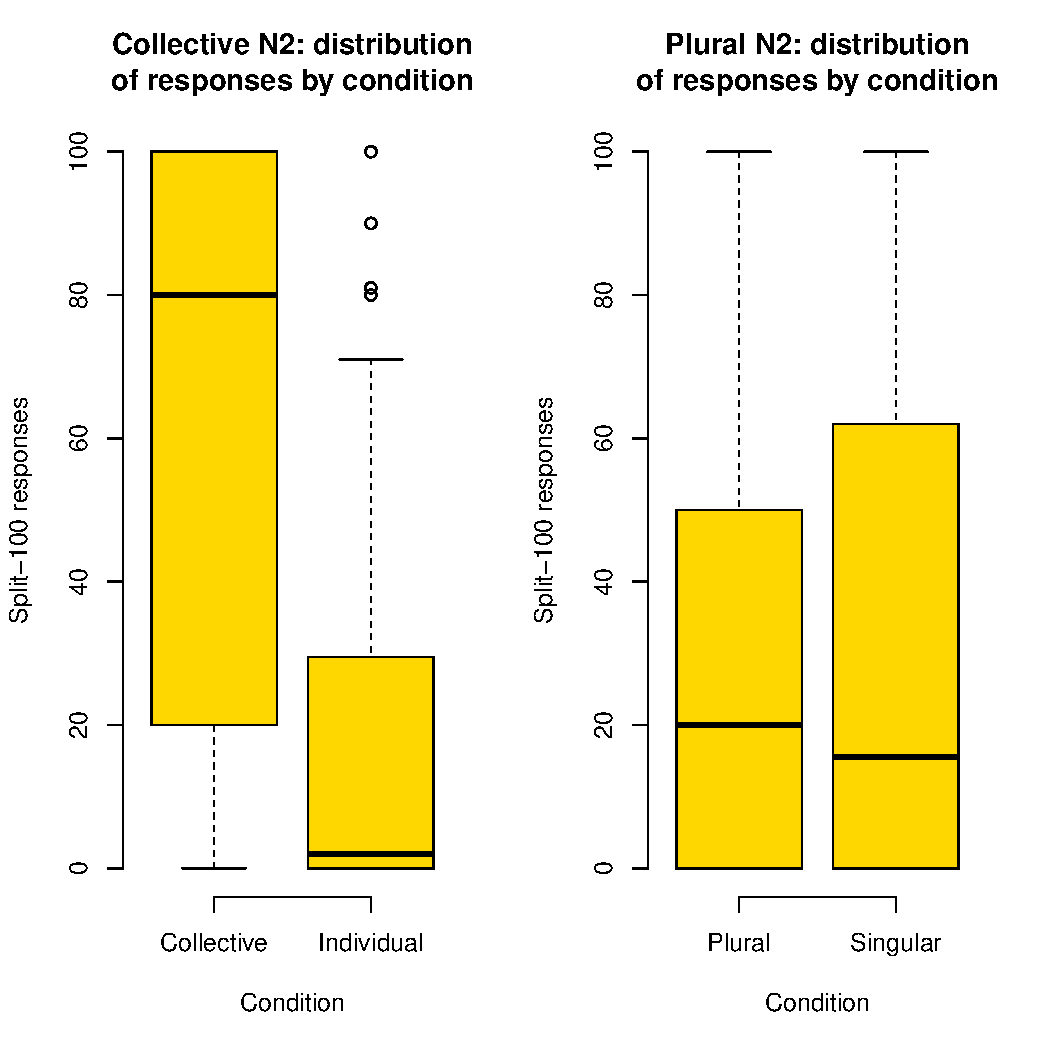
\includegraphics[width=\textwidth]{graphics/descriptive_by_condition}
  \caption{Descripitive results of the split-100 experiment}
  \label{fig:split100descriptive}
\end{figure}

\section*{Acknowledgments}

We would like to thank (in alphabetical order) Ulrike Sayatz for valuable discussions and comments.
Furthermore, we thank Ulrike Sayatz for helping us to recruit the participants for the experiments.
We are fully responsible for all residual adequacies, errors, and omissions.
Roland Schäfer's work on this project was funded in part by the \textit{Deutsche Forschungsgemeinschaft} (DFG, personal grant SCHA1916/1-1).


\printbibliography


\end{document}
